\section{Representations for a word}
\begin{itemize}
\item So far, we've basically had one representation of words, the word embeddings we've already learned:  Word2vec, GloVe, fastText.\footnote{These slides are partially based on the Stanford CS224N: Natural Language Processing with Deep Learning course: \url{http://web.stanford.edu/class/cs224n/}}.
\item These embeddings have a useful semi-supervised quality, as they can be learned from unlabeled corpora and used in our downstream task-oriented architectures (LSTM, CNN, Transformer).

\item However, they exhibit two problems.
\item  Problem 1: They always produce the same representation for a word type regardless of the context in which a word token occurs
\item  We might want very fine-grained word sense disambiguation
\item Problem 2: We just have one representation for a word, but words have different aspects, including semantics, syntactic behavior, and register/connotations

 

\end{itemize}

\section{Neural Language Models can produce Contextualized Embeddings}
\begin{itemize}
\item In a Neural Language Model (NLM), we immediately stuck word vectors (perhaps only trained on the corpus) through LSTM layers
\item  Those LSTM layers are trained to predict the next word.
\item  But these language models produce context-specific word representations in the hidden states of each position.

    \begin{figure}[h]
        	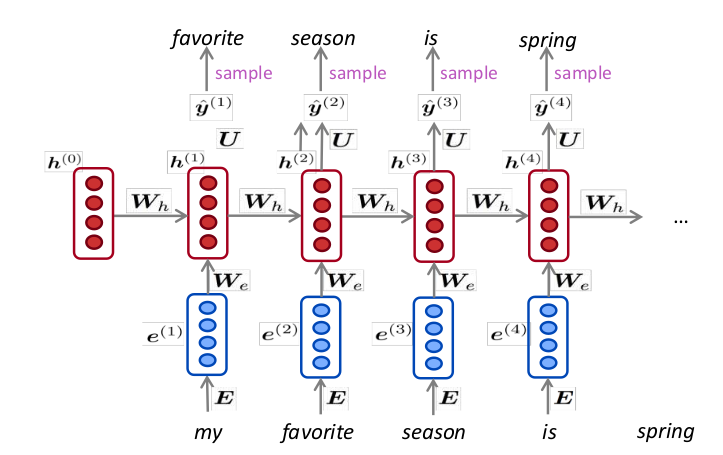
\includegraphics[scale = 0.4]{pics/lstm_nlm.png}
        \end{figure}  


\end{itemize}



\section{ELMo: Embeddings from Language Models}
\begin{itemize}
\item Idea: train a large language model (LM)  with a recurrent neural network and use its hidden states as ``contextualized word embeddings'' 
\cite{peters-etal-2018-deep}. 

\item ELMO is bidirectional LM with 2 biLSTM layers and around 100 million parameters.
\item  Uses character CNN to build initial word representation (only)
\item  2048 char n-gram filters and 2 highway layers, 512 dim projection
\item  User 4096 dim hidden/cell LSTM states with 512 dim projections to next input
\item  Uses a residual connection
\item  Parameters of token input and output (softmax) are tied.

\end{itemize}

    \begin{figure}[h]
        	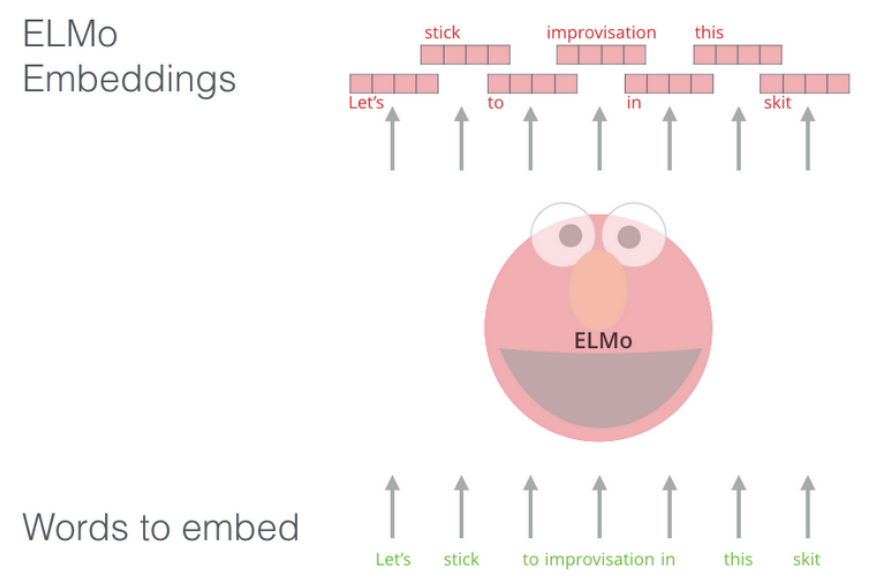
\includegraphics[scale = 0.29]{pics/elmo.png}
        \end{figure}  



\subsection{ELMo: Use with a task}
\begin{itemize}
\item First run biLM to get representations for each word.
\item Then let (whatever) end-task model use them.
\item  Freeze weights of ELMo for purposes of supervised model.
\item  Concatenate ELMo weights into task-specific model.


    \begin{figure}[h]
        	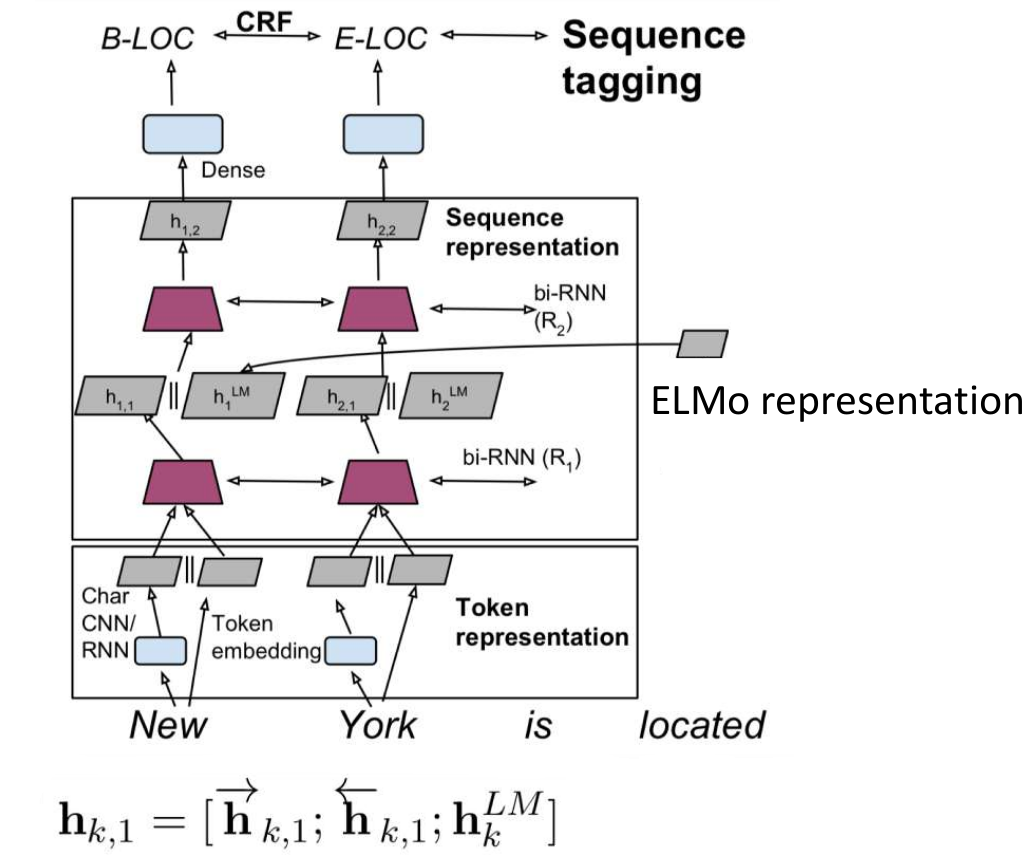
\includegraphics[scale = 0.25]{pics/elmo2.png}
        \end{figure}  

 

\end{itemize}

\paragraph{ELMo: Results}

    \begin{figure}[h]
        	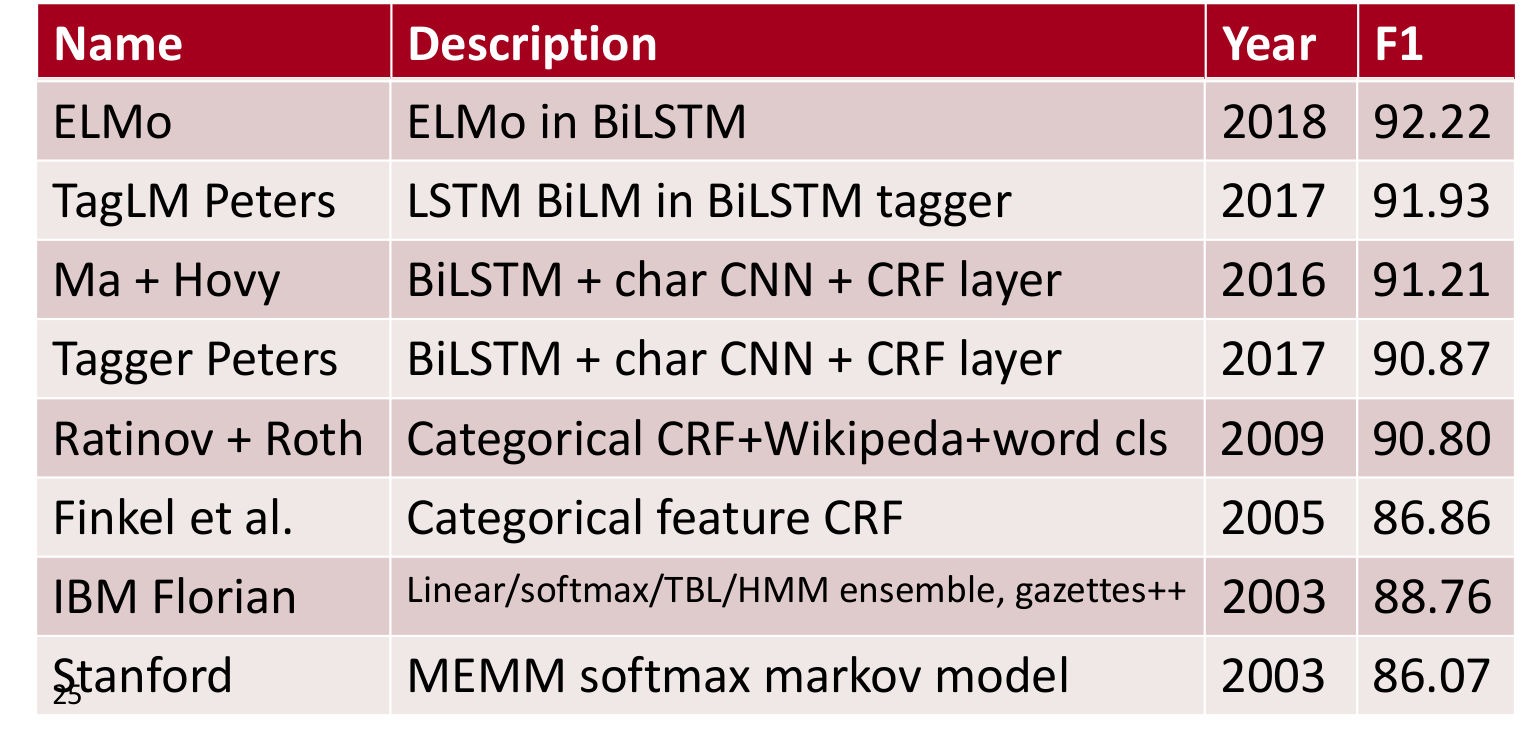
\includegraphics[scale = 0.25]{pics/elmo_results.png}
        \end{figure}  

 

\section{ULMfit}
\begin{itemize}
\item Howard and Ruder (2018) Universal Language Model Fine-tuning for Text Classification \cite{howard-ruder-2018-universal}. 
\item Same general idea of transferring NLM knowledge
\item  Here applied to text classification

\begin{figure}[h]
        	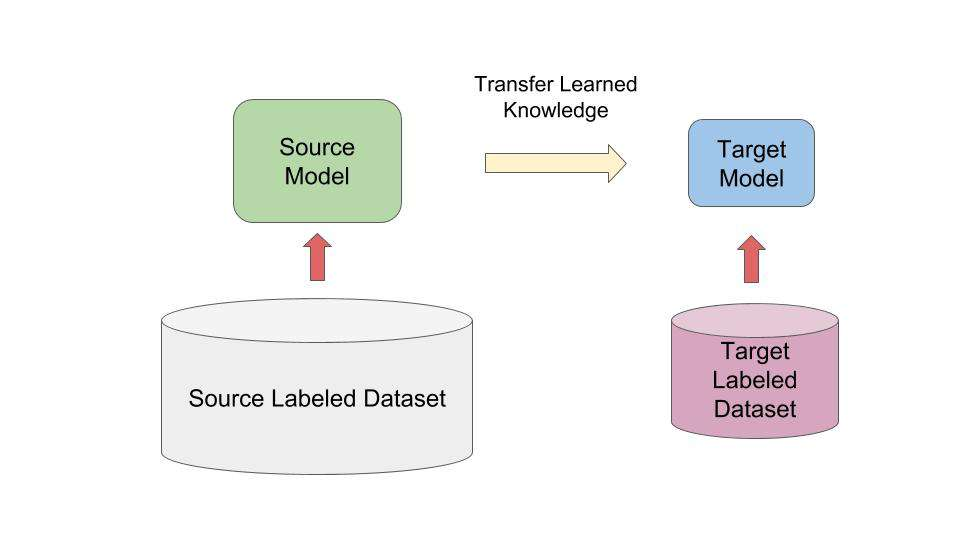
\includegraphics[scale = 0.29]{pics/ulmfit1.png}
        \end{figure}  

\item Train LM on big general domain corpus (use biLM)
\item Tune LM on target task data
\item Fine-tune as classifier on target task

\begin{figure}[h]
        	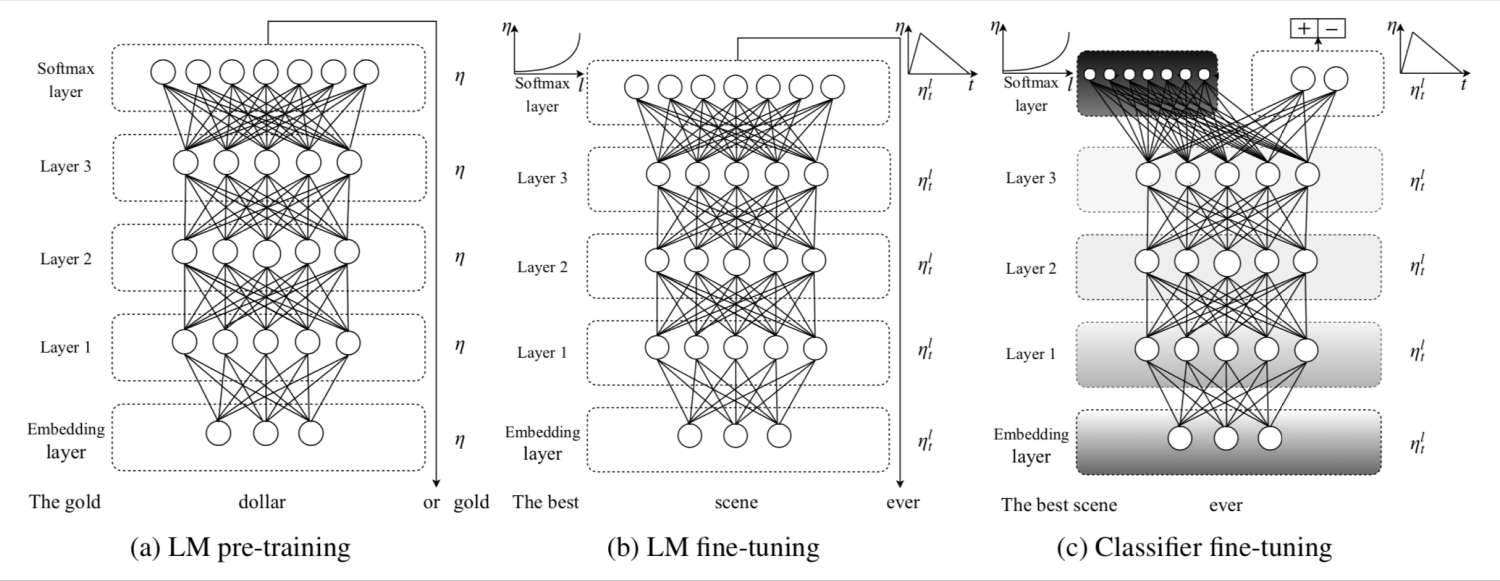
\includegraphics[scale = 0.2]{pics/ulmfit2.png}
        \end{figure}  

\end{itemize}



\subsection{ULMfit emphases}
\begin{itemize}
\item Use reasonable-size ``1 GPU'' language model not really huge one
\item A lot of care in LM fine-tuning
\item Different per-layer learning rates
\item Slanted triangular learning rate (STLR) schedule
\item Gradual layer unfreezing and STLR when learning classifier
\item Classify using concatenation $[h_T, $maxpool$(h),$meanpool$(h)]$

\begin{figure}[h]
        	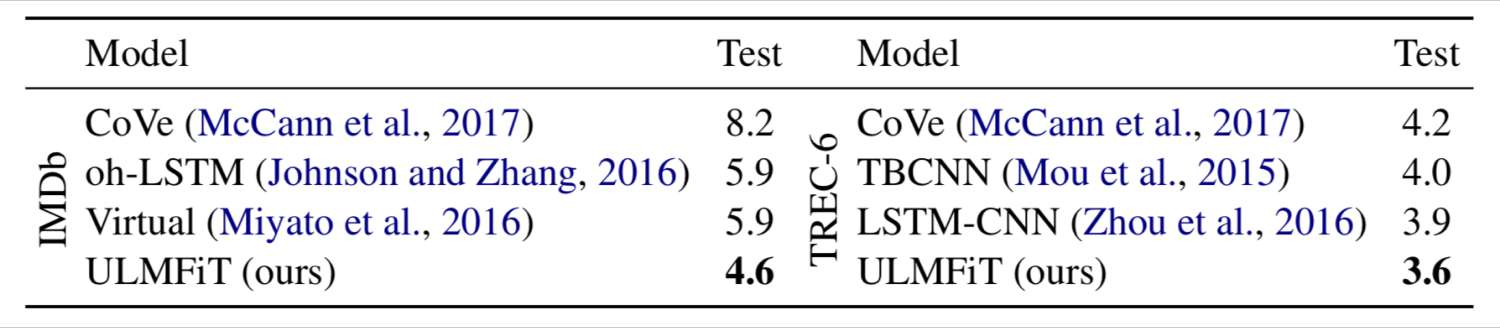
\includegraphics[scale = 0.2]{pics/ulmfit3.png}
        	Text classifier error rates
        \end{figure}  

\end{itemize}


\subsection{ULMfit transfer learning}

\begin{figure}[h]
        	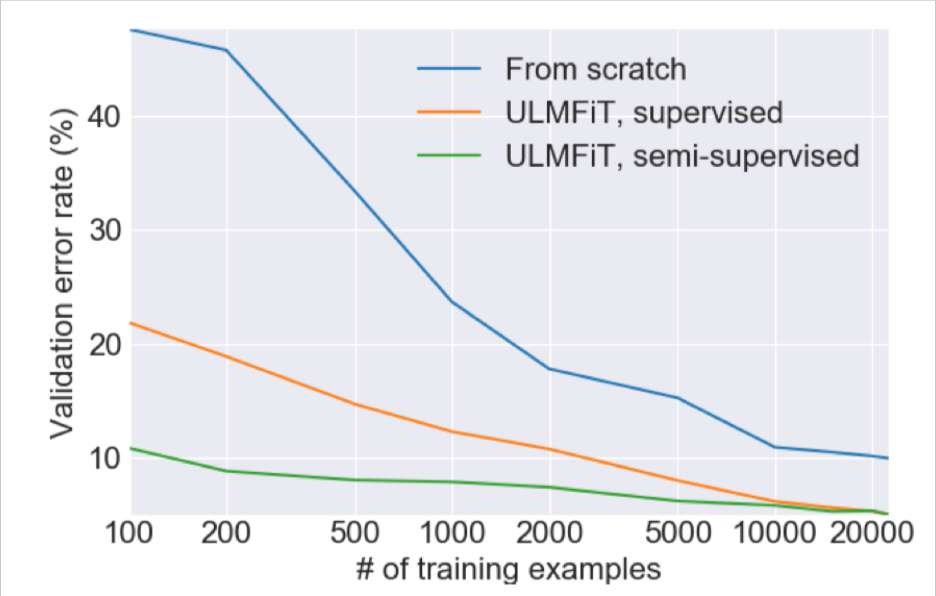
\includegraphics[scale = 0.3]{pics/ulmfit4.png}
        \end{figure}  



\section{Let’s scale it up!}


     \begin{figure}[h]
        	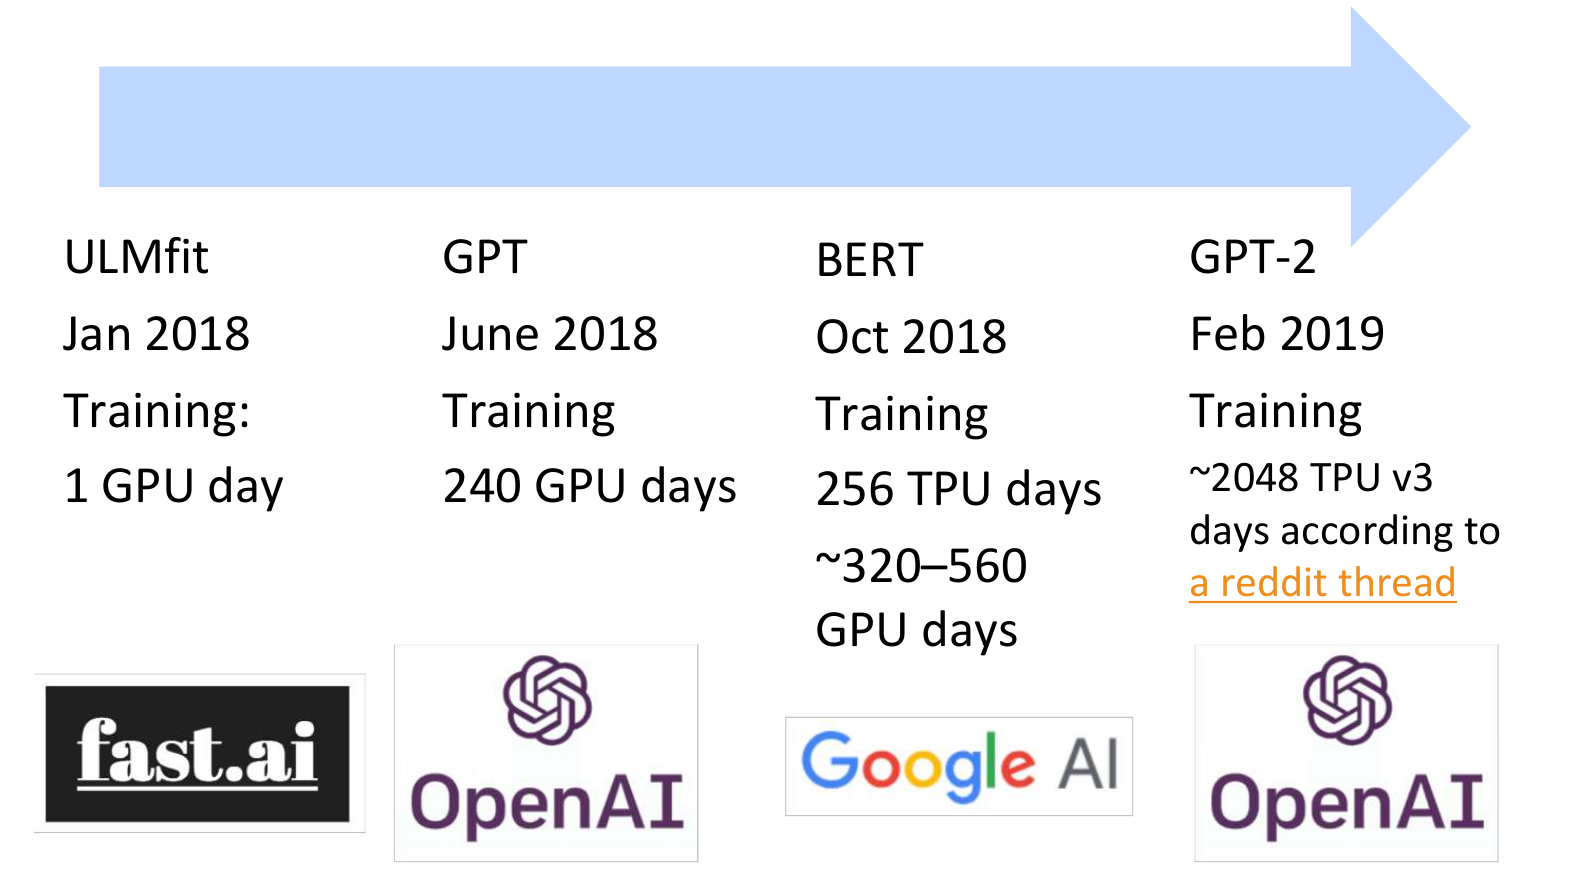
\includegraphics[scale = 0.28]{pics/llmscale.png}
        \end{figure}  



     \begin{figure}[h]
        	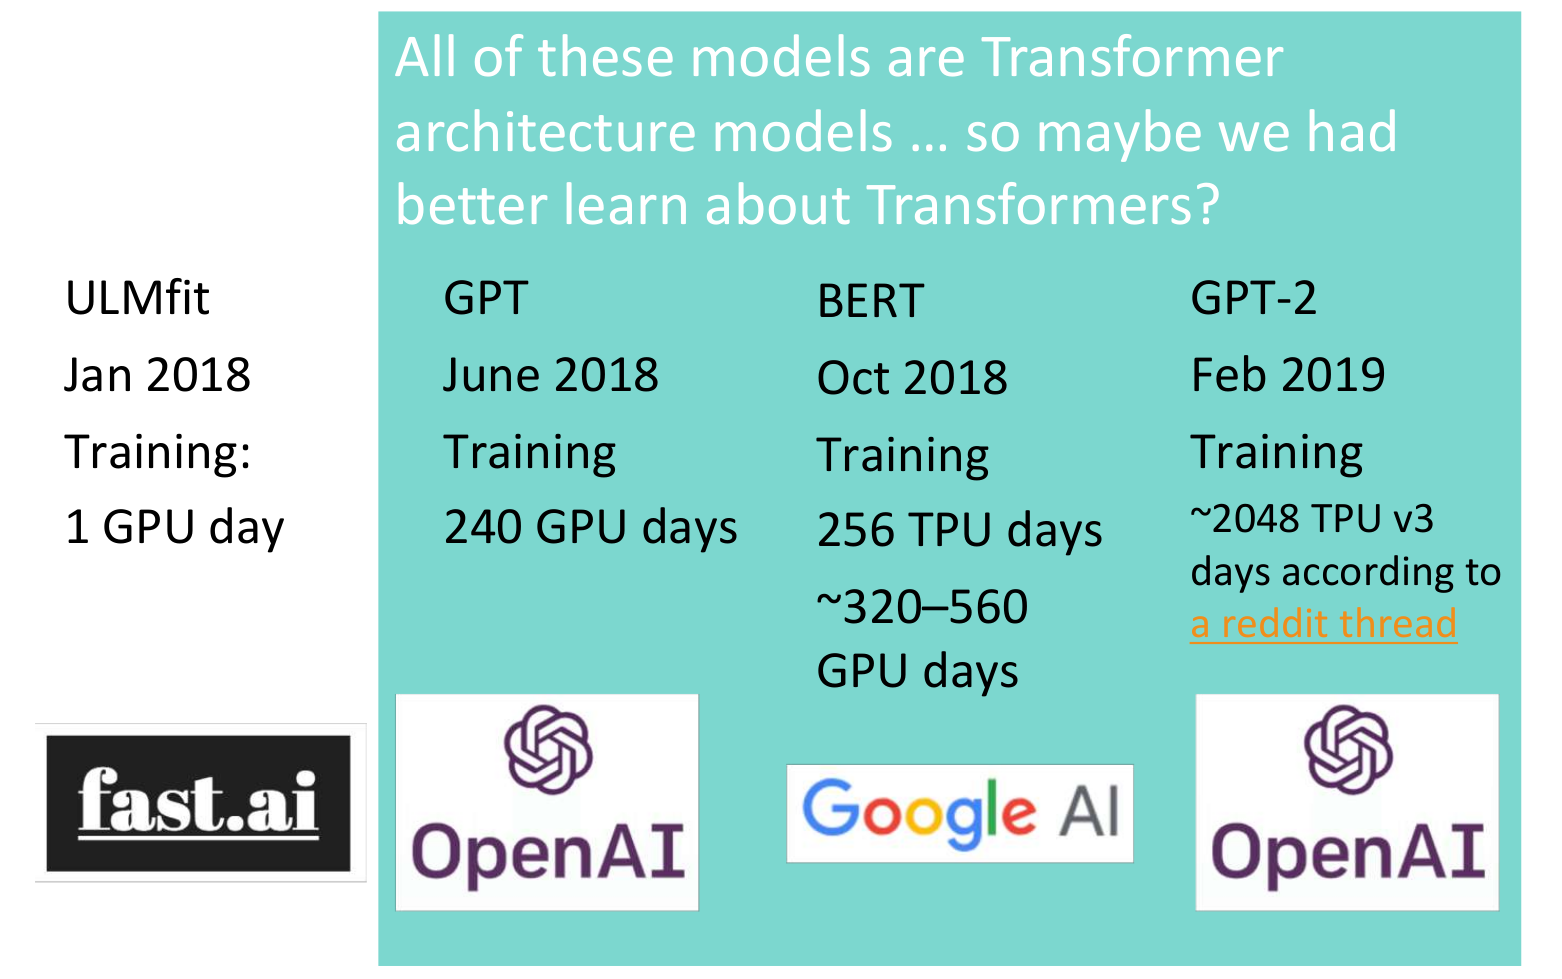
\includegraphics[scale = 0.28]{pics/llmscale_trans.png}
        \end{figure}  


\section{BERT (Bidirectional Encoder Representations from Transformers)}
\begin{itemize}
\item Idea: combine ideas from ELMO, ULMFit and the Transformer \cite{kenton2019bert}.
\item How: Train a large model (335 million parameters) from a large unlabeled corpus using a Transformer encoder and then fine-tune it for other downstream tasks.
\item The parallelizable properties of the Transformer (unlike RNNs, which must be processed sequentially) allow the model to scale to more parameters.
\item This model is related but a little bit different from a standard Language Model.

     \begin{figure}[h]
        	
\includegraphics[scale = 0.4]{pics/bert.png}
        \end{figure}  
\item BERT  doesn't predict the next word in a sentence like a traditional language model, but rather learns utilizes a ``\textbf{masked language modeling}'' (MLM) objective during pre-training.

\item In MLM, random words in a sentence are masked and the model is trained to predict those masked words based on the surrounding context.
\item BERT also incorporates a ``\textbf{next sentence prediction}'' task, where pairs of sentences are fed to the model, and it learns to predict whether the second sentence follows the first in the original text.
\item \textbf{Fine-tuning} BERT involves adding a task-specific layer on top of the pre-trained model and training it on a labeled dataset for the target task.
\item BERT achieved state-of-the-art results at the time of its release on NLP tasks, including sentence classification, named entity recognition, question answering, and more.





\end{itemize}


\section{Masked Language Modeling and Next Sentence Prediction}
\begin{itemize}
\item MLM: Mask out k\% of the input words, and then predict the masked words
\item They always use k = 15\%.

     \begin{figure}[h]
        	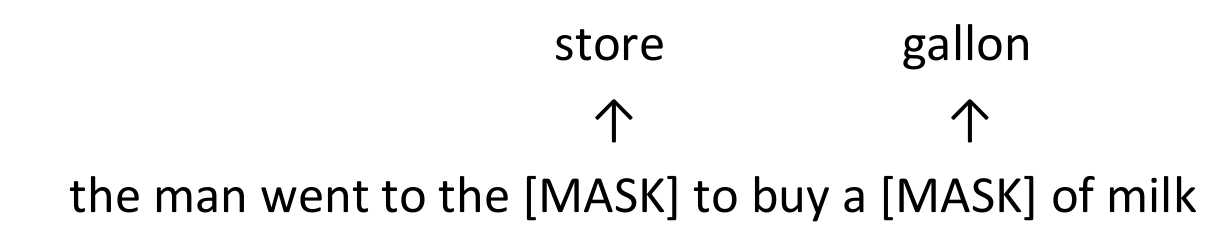
\includegraphics[scale = 0.3]{pics/MLM.png}
        \end{figure}  

\item Too little masking: Too expensive to train
\item Too much masking: Not enough context

\item Next sentence prediction: To learn relationships between sentences, predict whether
Sentence B is actual sentence that proceeds Sentence A, or a random sentence

 \begin{figure}[h]
        	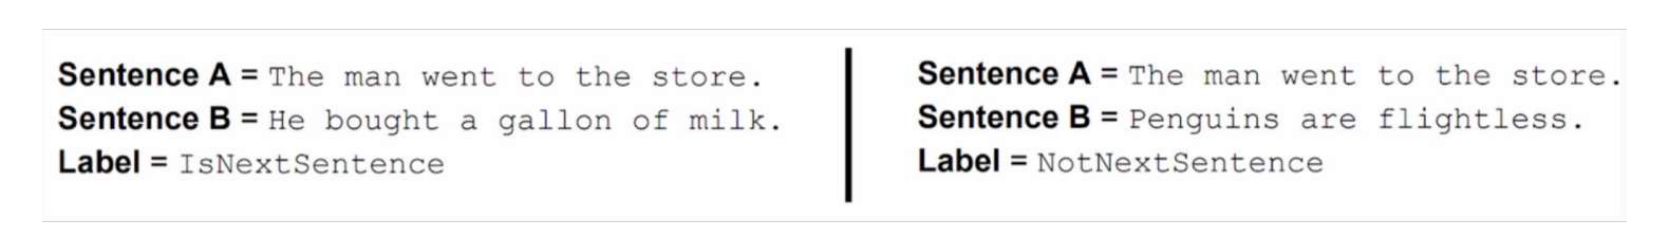
\includegraphics[scale = 0.23]{pics/NSP.png}
        \end{figure}  



\end{itemize}


\section{BERT sentence pair encoding}
\begin{itemize}
\item Token embeddings: Words are divided into smaller units called word pieces, and each word piece is assigned a token embedding.
\item BERT learns a segmented embedding [SEP] to differentiate between the two sentences in a pair.
\item BERT utilizes positional embeddings to capture the position of each word within the sentence.

 \begin{figure}[h]
        	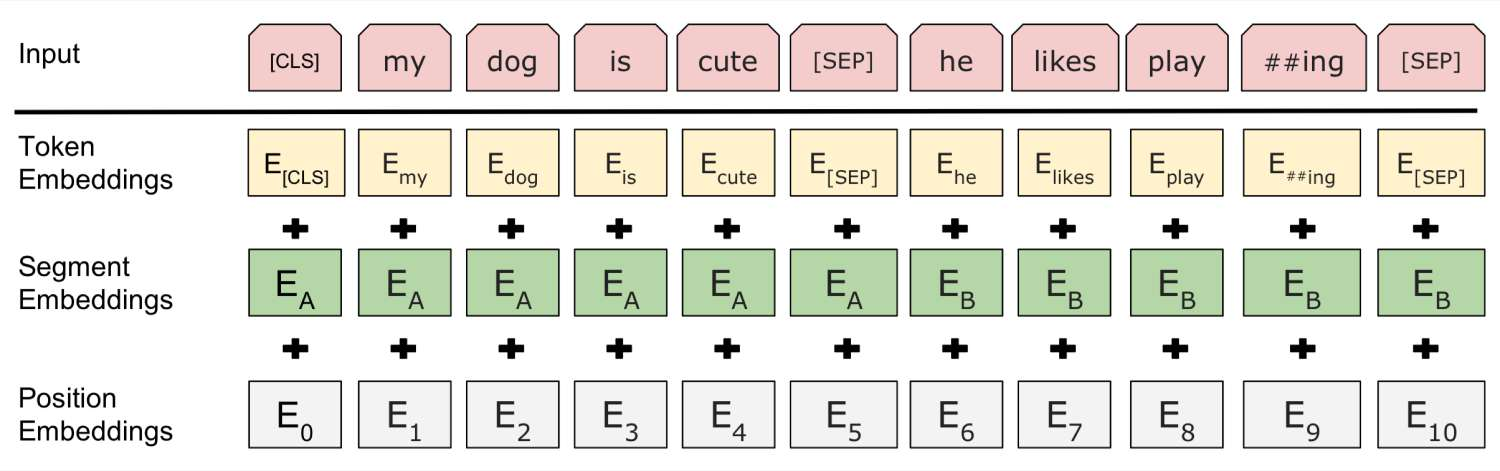
\includegraphics[scale = 0.18]{pics/BSPE.png}
        \end{figure}  



\end{itemize}


\section{BERT Model Architecture and Training}
\begin{itemize}
\item BERT is based on the Transformer encoder.
\item The multi-headed self-attention block of the Transformer  allows BERT to consider long-distance context effectively.
\item The use of self-attention also enables efficient computations on GPU/TPU, with only a single multiplication per layer.
\item BERT was trained on a large amount of unlabeled text data from Wikipedia and BookCorpus.
\item Two different model sizes were trained:
\begin{enumerate}\scriptsize{
\item BERT-Base: 12 layers, 768 hidden units, and 12 attention heads.
\item BERT-Large: 24 layers, 1024 hidden units, and 16 attention heads.}
\end{enumerate}
\item The training process involved utilizing 4x4 or 8x8 TPU (Tensor Processing Unit) configurations for faster computation.
\item Training BERT models took approximately 4 days to complete.
\end{itemize}


\section{BERT model fine tuning}
\begin{itemize}
\item Fine-tuning involves customizing the pre-trained BERT model for specific tasks.
\item To fine-tune BERT, we add a task-specific layer on top of the pre-trained BERT model.
\item The task-specific layer can vary depending on the task at hand, such as sequence labeling or sentence classification.
\item We train the entire model, including the pre-trained BERT and the added task-specific layer, for the specific task.
\end{itemize}

 \begin{figure}[h]
        	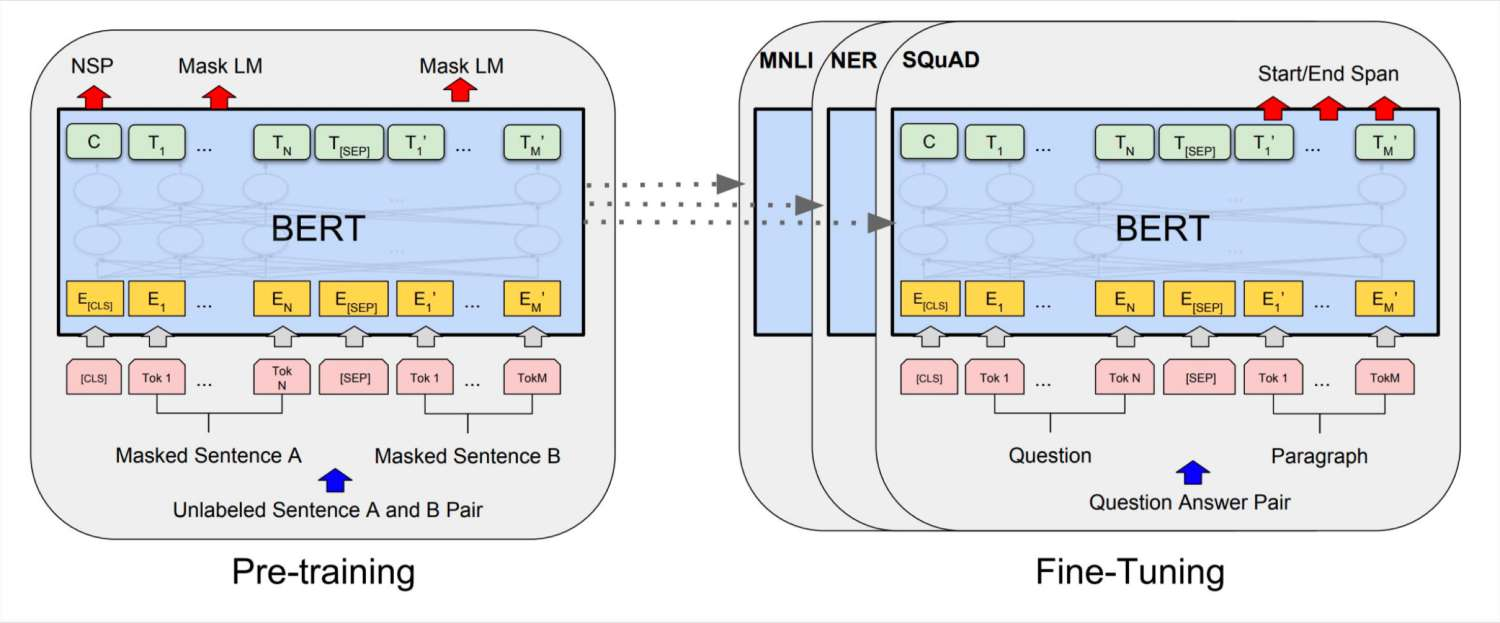
\includegraphics[scale = 0.2]{pics/BERTFineTuning.png}
        \end{figure}  



\subsection{BERT results on GLUE tasks}
\begin{itemize}
 \item BERT was massively popular and hugely versatile; finetuning BERT led to new state-of-
the-art results on a broad range of tasks.
\item BERT's performance was assessed using the GLUE benchmark, a collection of diverse NLP tasks.
\item The GLUE benchmark primarily consists of natural language inference tasks, but also includes sentence similarity and sentiment analysis tasks.
\end{itemize}

\textbf{Example Task: MultiNLI (Natural Language Inference)}
\begin{itemize}
\item Premise: "Hills and mountains are especially sanctified in Jainism."
\item Hypothesis: "Jainism hates nature."
\item Label: Contradiction
\end{itemize}

\textbf{Example Task: CoLa}
\begin{itemize}
\item Sentence: "The wagon rumbled down the road."
\item Label: Acceptable
\end{itemize}
\begin{itemize}
\item Sentence: "The car honked down the road."
\item Label: Unacceptable
\end{itemize}

 \begin{figure}[h]
        	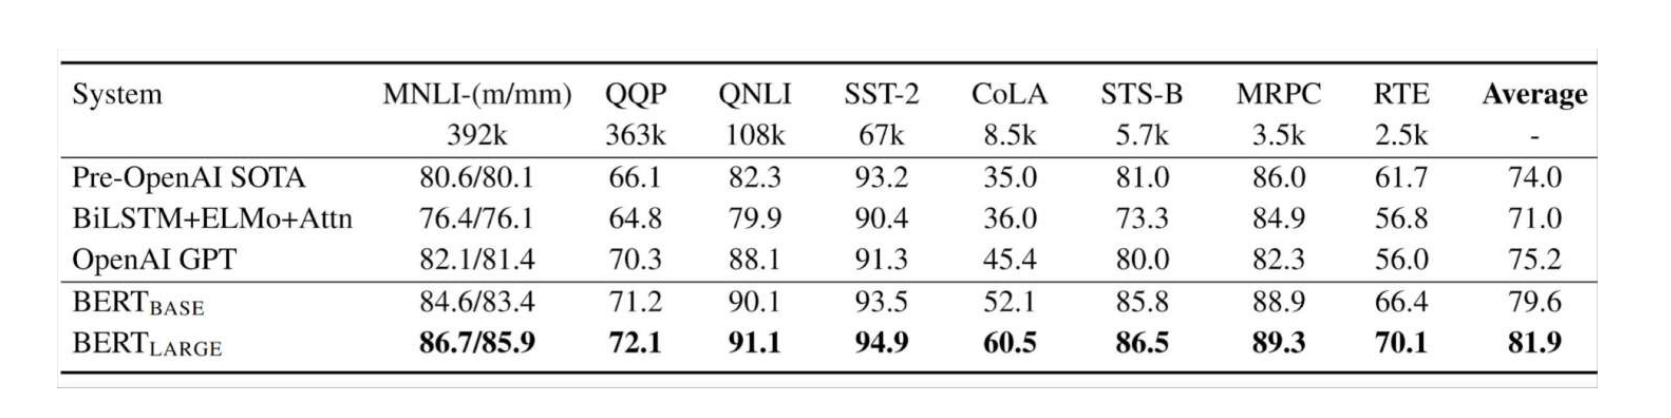
\includegraphics[scale = 0.26]{pics/BERTGLUE.png}
        \end{figure}  


\begin{itemize}
\item QQP: Quora Question Pairs (detect paraphrase questions)
\item QNLI: natural language inference over question answering data
\item SST-2: sentiment analysis 
\item CoLA: corpus of linguistic acceptability (detect whether sentences are grammatical.)
\item STS-B: semantic textual similarity
\item MRPC: microsoft paraphrase corpus
\item  RTE: a small natural language inference corpus
\end{itemize}



\subsection{BERT Effect of pre-training task}


 \begin{figure}[h]
        	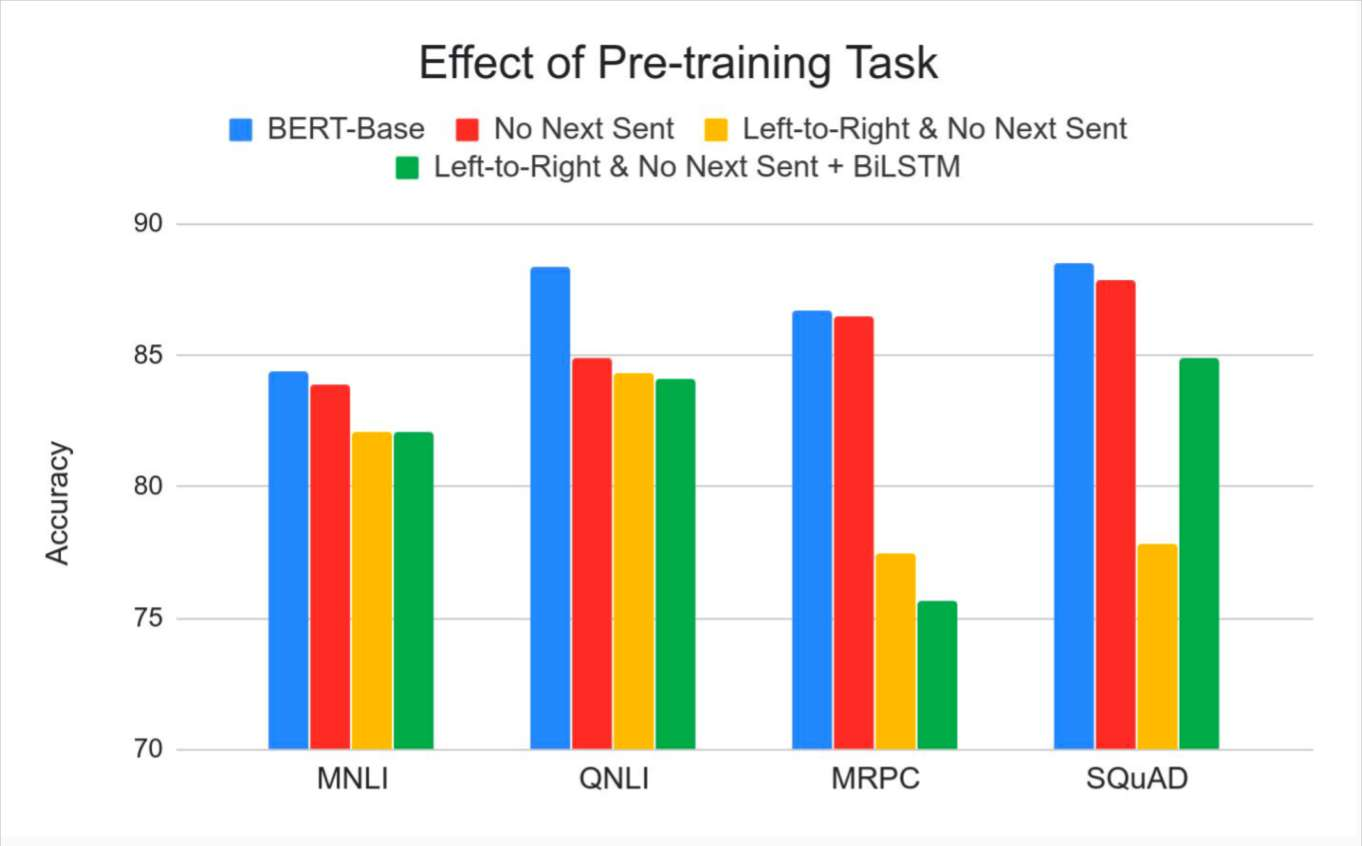
\includegraphics[scale = 0.2]{pics/BERTeffect.png}
        \end{figure}  


\section{Pre-training decoders GPT and GPT-2}

\begin{itemize}
\item Contemporary to BERT, OpenAI introduced an alternative approach called Generative Pretrained Transformer (GPT) \cite{radford2018improving}.
\item The idea behind GPT is to train a large standard language model using the generative part of the Transformer, specifically the decoder.
\item GPT is a Transformer decoder with 12 layers and 117 million parameters.
\item It has 768-dimensional hidden states and 3072-dimensional feed-forward hidden layers.
\item GPT utilizes byte-pair encoding with 40,000 merges to handle subword units.
\item GPT was trained on BooksCorpus, which consists of over 7,000 unique books.
\item OpenAI later introduced GPT-2, a larger version with 1.5 billion parameters, trained on even more data.
\item GPT-2 has been shown to generate relatively convincing samples of natural language.
\end{itemize}


\paragraph{GPT-2 language model (cherry-picked) output}
\textbf{Human provided prompt}:

In a shocking finding, scientist discovered a herd of unicorns living in a remote, previously unexplored valley, in the Andes Mountains. Even more surprising to the researchers was the fact that the unicorns spoke perfect English. \\ 
\textbf{Model Completition}: \\ 

The scientist named the population, after their distinctive horn, Ovid’s Unicorn. These four-horned, silver-white unicorns were previously unknown to science.

Now, after almost two centuries, the mystery of what sparked this odd phenomenon is finally solved.

Dr. Jorge Pérez, an evolutionary biologist from the University of La Paz, and several companions, were exploring the Andes Mountains when they found a small valley, with no other animals or humans. Pérez noticed that the valley had what appeared to be a natural fountain, surrounded by two peaks of rock and silver snow.



\section{What kinds of things does pretraining learn?}

\begin{itemize}
\item Stanford University is located in \_\_\_\_\_, California. [Trivia]
\item I put \_\_\_\_\_ fork down on the table. [syntax]
\item The woman walked across the street, checking for traffic over \_\_\_\_\_ shoulder. [coreference]
 \item I went to the ocean to see the fish, turtles, seals, and \_\_\_\_\_. [lexical semantics/topic]
\item Overall, the value I got from the two hours watching it was the sum total of the popcorn and the drink. The movie was \_\_\_\_\_. [sentiment]
\item Iroh went into the kitchen to make some tea. Standing next to Iroh, Zuko pondered his destiny. Zuko left the \_\_\_\_\_. [some reasoning – this is harder]
\item I was thinking about the sequence that goes 1, 1, 2, 3, 5, 8, 13, 21, \_\_\_\_\_ [some basic arithmetic; they don’t learn the Fibonnaci sequence]
\end{itemize}


\section{Phase Change: GPT-3 (2020)}
\begin{itemize}
\item GPT-3 is another Transformer-based Language Model (LM) that pushed the boundaries with nearly 200 billion parameters, making it the largest model at the time \cite{brown2020language}.
\item It was trained on a massive corpus consisting of nearly 500 billion words.
\item \textbf{In-context learning}: GPT-3 demonstrated the ability to solve various natural language processing (NLP) tasks using \textbf{zero-shot}, \textbf{one-shot} and \textbf{few-shot learning}.
\item The key to this capability lies in the prompt or context provided to GPT-3.
\item GPT-3 demonstrated the ability to solve various tasks without performing gradient updates to the base model.
\end{itemize}

 \begin{figure}[h]
        	
\includegraphics[scale = 0.08]{pics/gpt3.png}
        \end{figure}  




\section{Zero-shot, One-shot, and Few-shot Learning with GPT-3}
\begin{itemize}
\item \textbf{Zero-shot learning}: With zero-shot learning, GPT-3 can tackle tasks  without any specific training. It achieves this by providing a prompt or instruction to guide its generation process. For example, by providing GPT-3 with a prompt like, ``Translate this English sentence to French,'' it can generate the translated sentence without any explicit training for translation tasks.
\item \textbf{One-shot learning}: In one-shot learning, GPT-3 can perform a task by adding a single input-output pair to the instruction.
\item \textbf{Few-shot learning}: similar idea but providing a limited number input-output pairs after the instruction in the prompt.
\end{itemize}

 \begin{figure}[h]
        	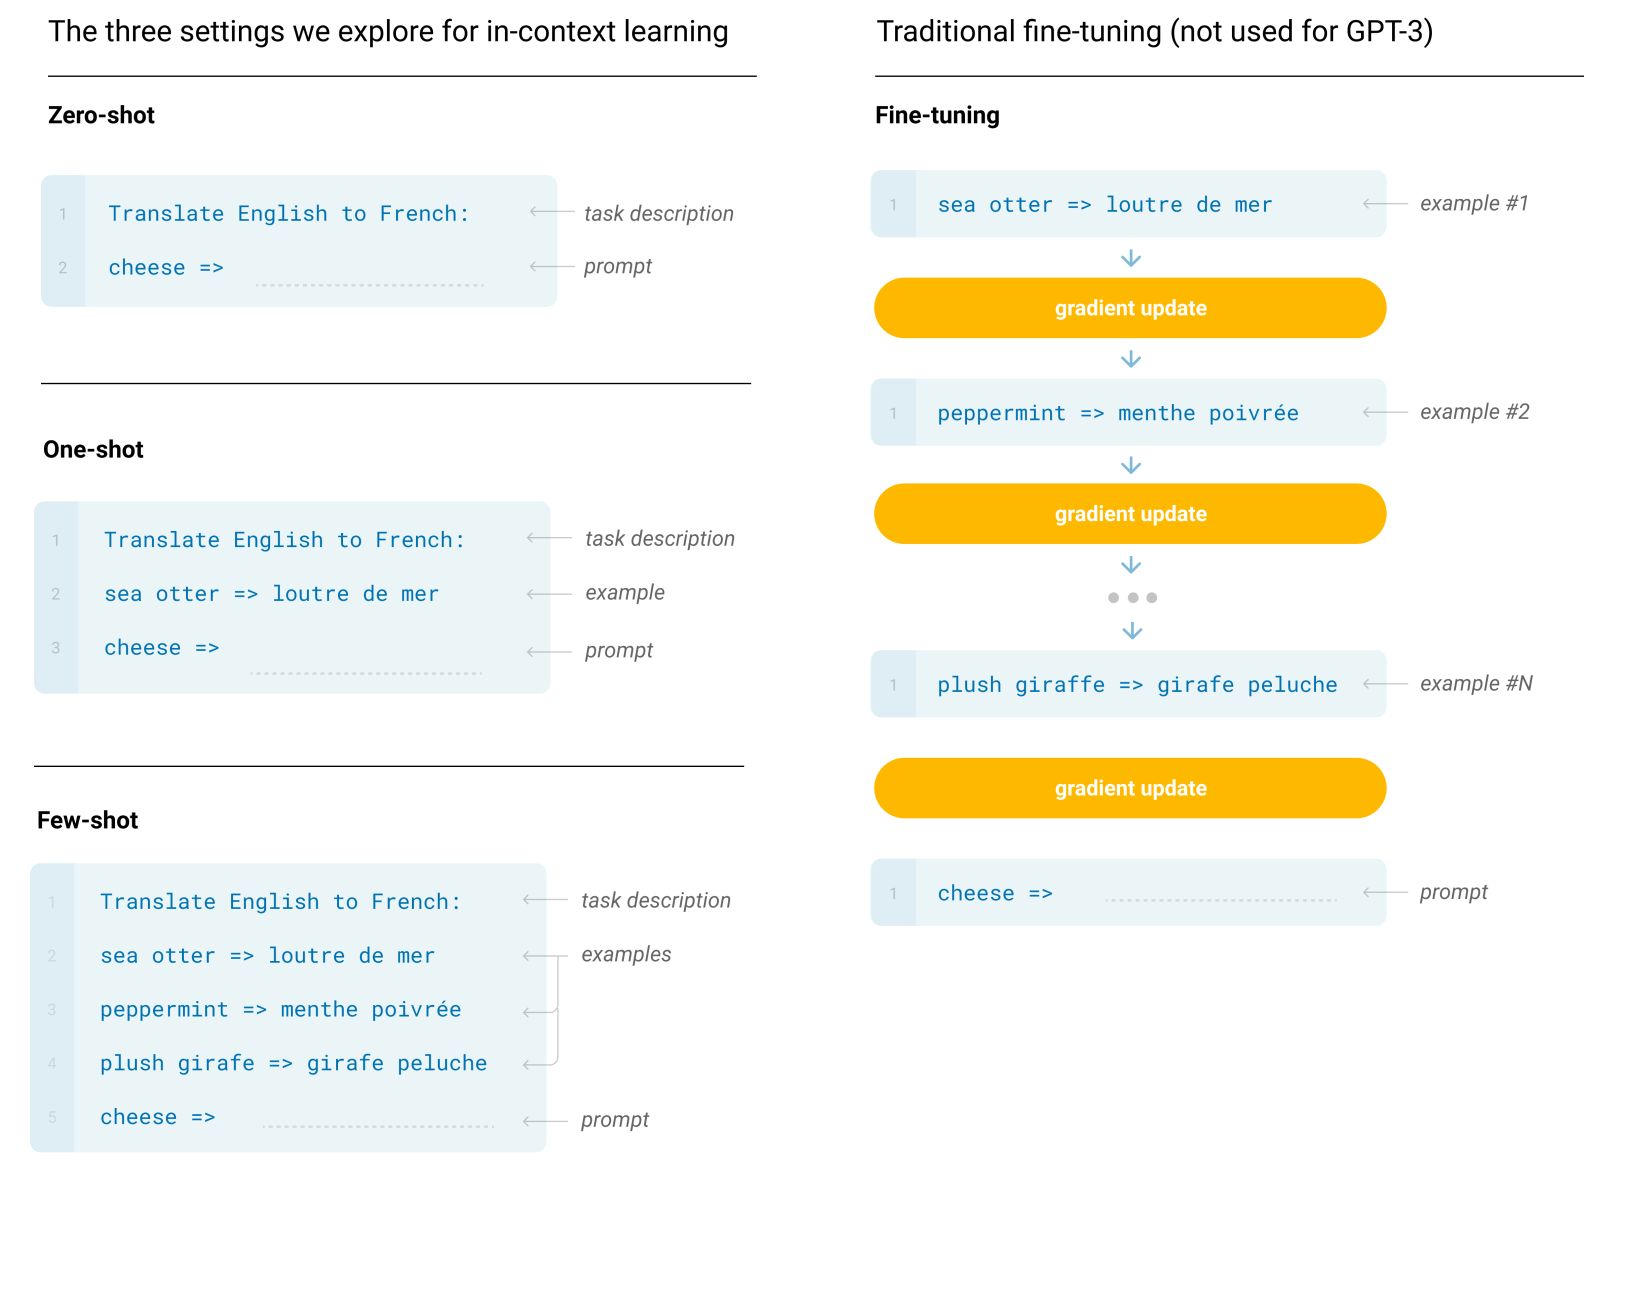
\includegraphics[scale = 0.18]{pics/zeroonefew.png}
        \end{figure}  



GPT-3 Few-shot Learning Results
 \begin{figure}[h]
        	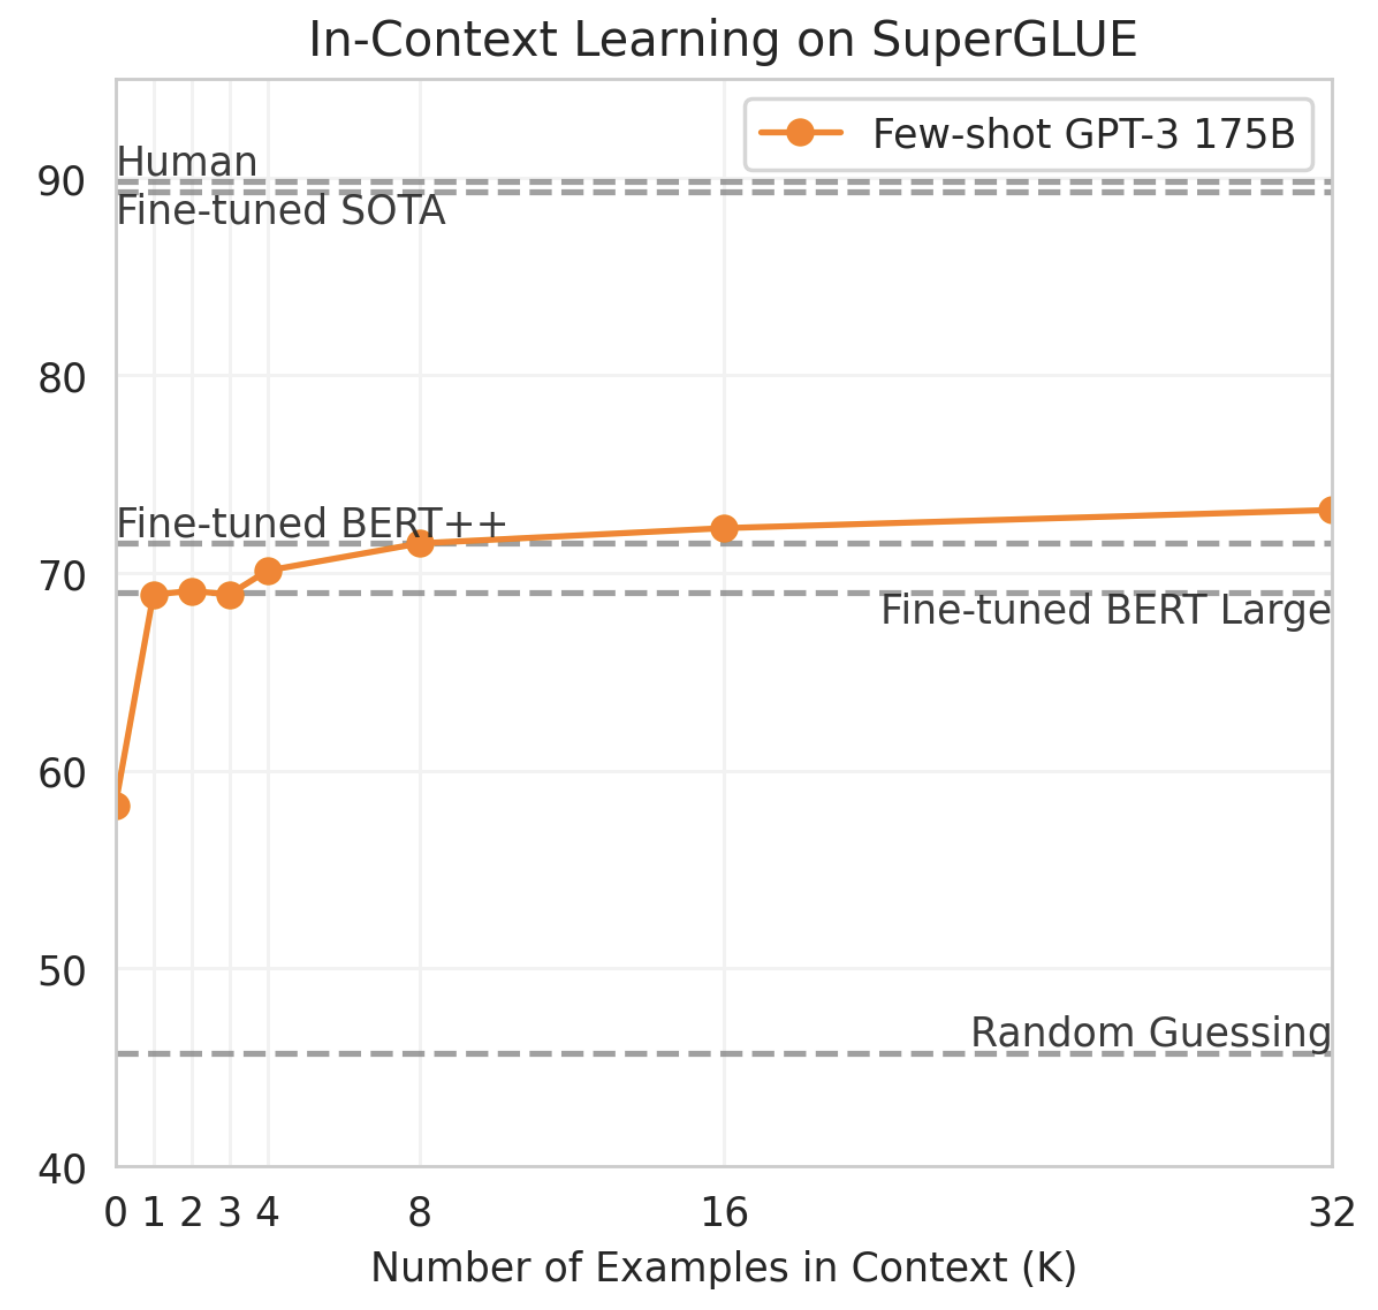
\includegraphics[scale = 0.15]{pics/fewshotresults.png}
        \end{figure}




\section{Chain-of-thought Prompting}
\begin{itemize}
\item Chain-of-thought prompting is a simple mechanism for eliciting multi-step rea-
soning behavior in large language models.
\item  Idea: augment each exemplar in few-shot prompting with a chain of thought for an associated answer \cite{wei2022chain}
\end{itemize}
 \begin{figure}[h]
        	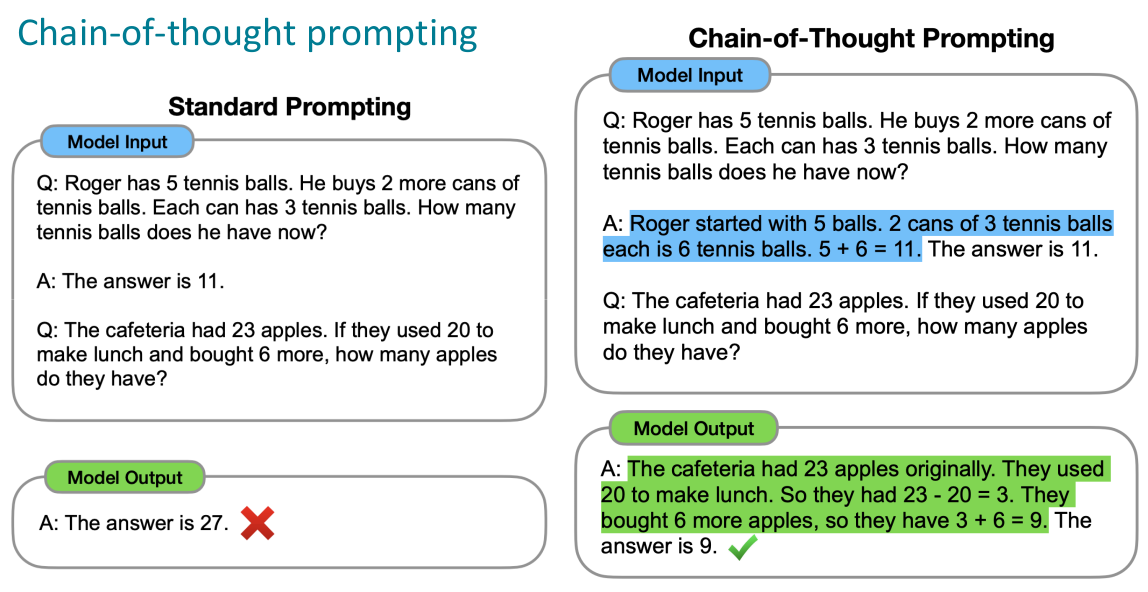
\includegraphics[scale = 0.3]{pics/chainoftought.png}
        \end{figure}



\section{Language Models as User Assitants (or Chatbots)}

\begin{itemize}
\item Autoregressive Large Language Models are not aligned with user intent \cite{ouyang2022training}


 \begin{figure}[h]
        	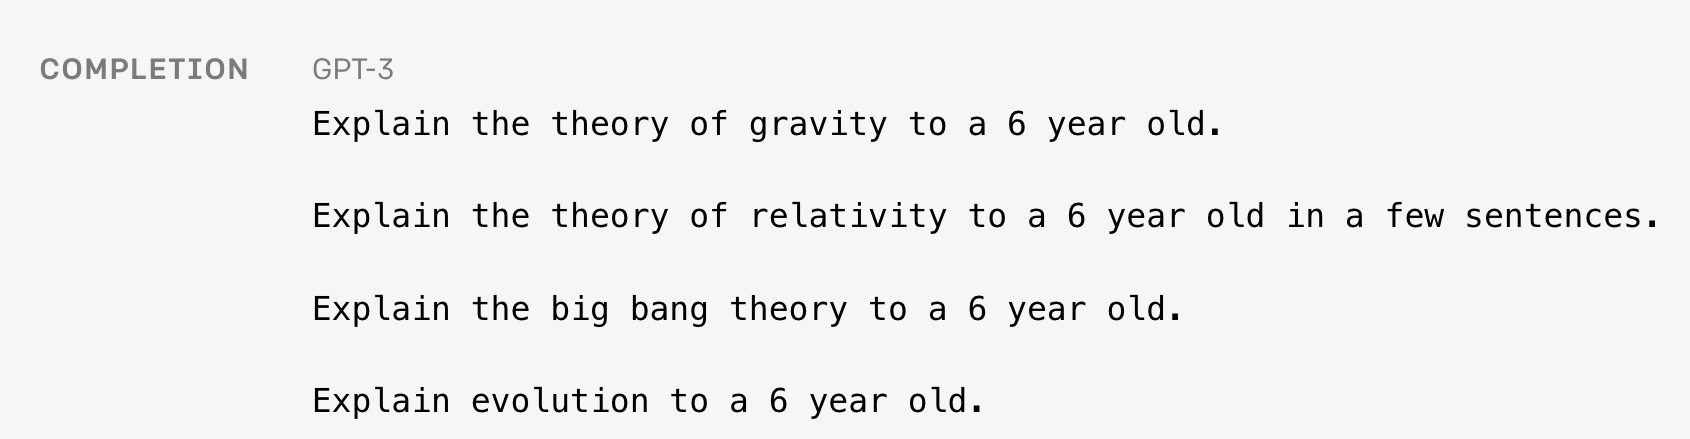
\includegraphics[scale = 0.34]{pics/lmnotuserassistant.png}
        \end{figure}

\item Solution: align the language model with user intent via fine-tuning.


\end{itemize}




\subsection{LaMDA: Language Models for Dialog Applications}
\begin{itemize}
\item LaMDA is a language model developed by Google based on Transformer optimized for open domain dialog \cite{thoppilan2022lamda}.
\item It has 137 billion parameters and is trained on 1.56 billion words.
\item It is initially pre-trained in the same way as traditional language models (predicting words) with language models (predicting words) with a strong focus on dialog data.
\item It is then fine-tuned to generate responses with respect to several other criteria.
\item In order to fit LaMBDA to all these criteria they worked with a large number of crowd-workers.
\item These are people who manually labeled conversations from the pre-trained model.
\end{itemize}


 \begin{figure}[h]
        	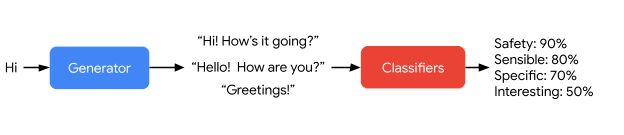
\includegraphics[scale = 0.5]{pics/lambda.png}
        \end{figure}


\paragraph{LaMDA Optimization Criteria}
\textbf{Quality}
\begin{itemize}
\item Sensibleness: give meaningful answers.
\item Specificity: avoid vague answers.
\item Interestingness: give insightful, unexpected or witty answers.
\end{itemize}

\textbf{Safety}
\begin{itemize}
\item Avoid violent language.
\item Avoid hate speech.
\item Avoid stereotyped speech.
\end{itemize}

\textbf{Groundedness and Informativity}
\begin{itemize}
\item Avoid giving answers not validated by external sources.
\item Optimize the fraction of responses that can be validated in authoritative sources using search engines.

\end{itemize}

\paragraph{LaMDA Evaluation}
\begin{itemize}
\item The system is compared with the original pre-trained PT model and human judgments.
\item The evaluation is done by another group of people through questionnaires.
\end{itemize}
 \begin{figure}[h]
        	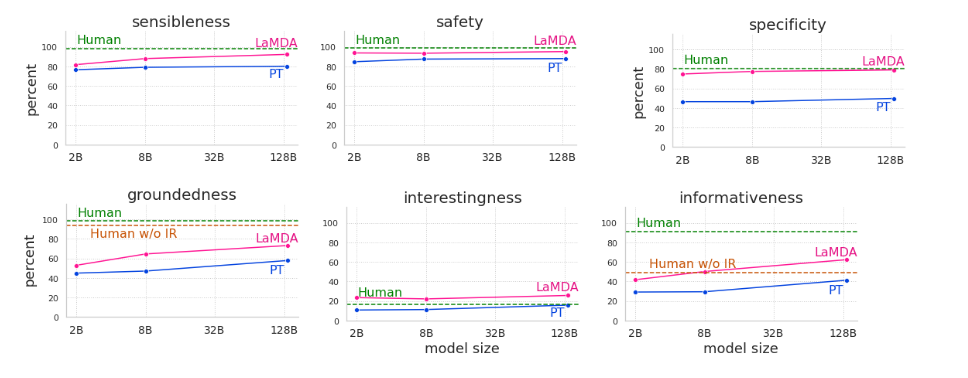
\includegraphics[scale = 0.45]{pics/lambdaresults.png}
        \end{figure}



\section{ChatGPT and RLHF}
\begin{itemize}
\item Model similar to LaMDA launched by OpenAI at the end of 2022.
\item It also uses Crowdsourcing to improve its responses, but its fine-tuning process uses Reinforcement Learning (RL), a different learning paradigm from supervised learning.
\item In particular, it uses Reinforcement Learning from Human Feedback (RLHF) \cite{ouyang2022training}.
\item It builds a preference model that assigns a score to a generated sentence and adjusts the language model accordingly.
\end{itemize}

\begin{figure}[h]
	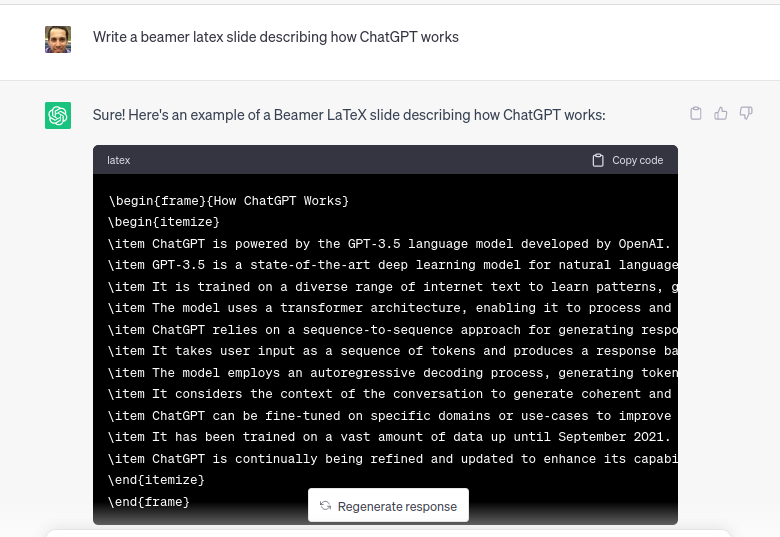
\includegraphics[scale = 0.25]{pics/chatgpt.png}
\end{figure}




 \begin{figure}[h]
        	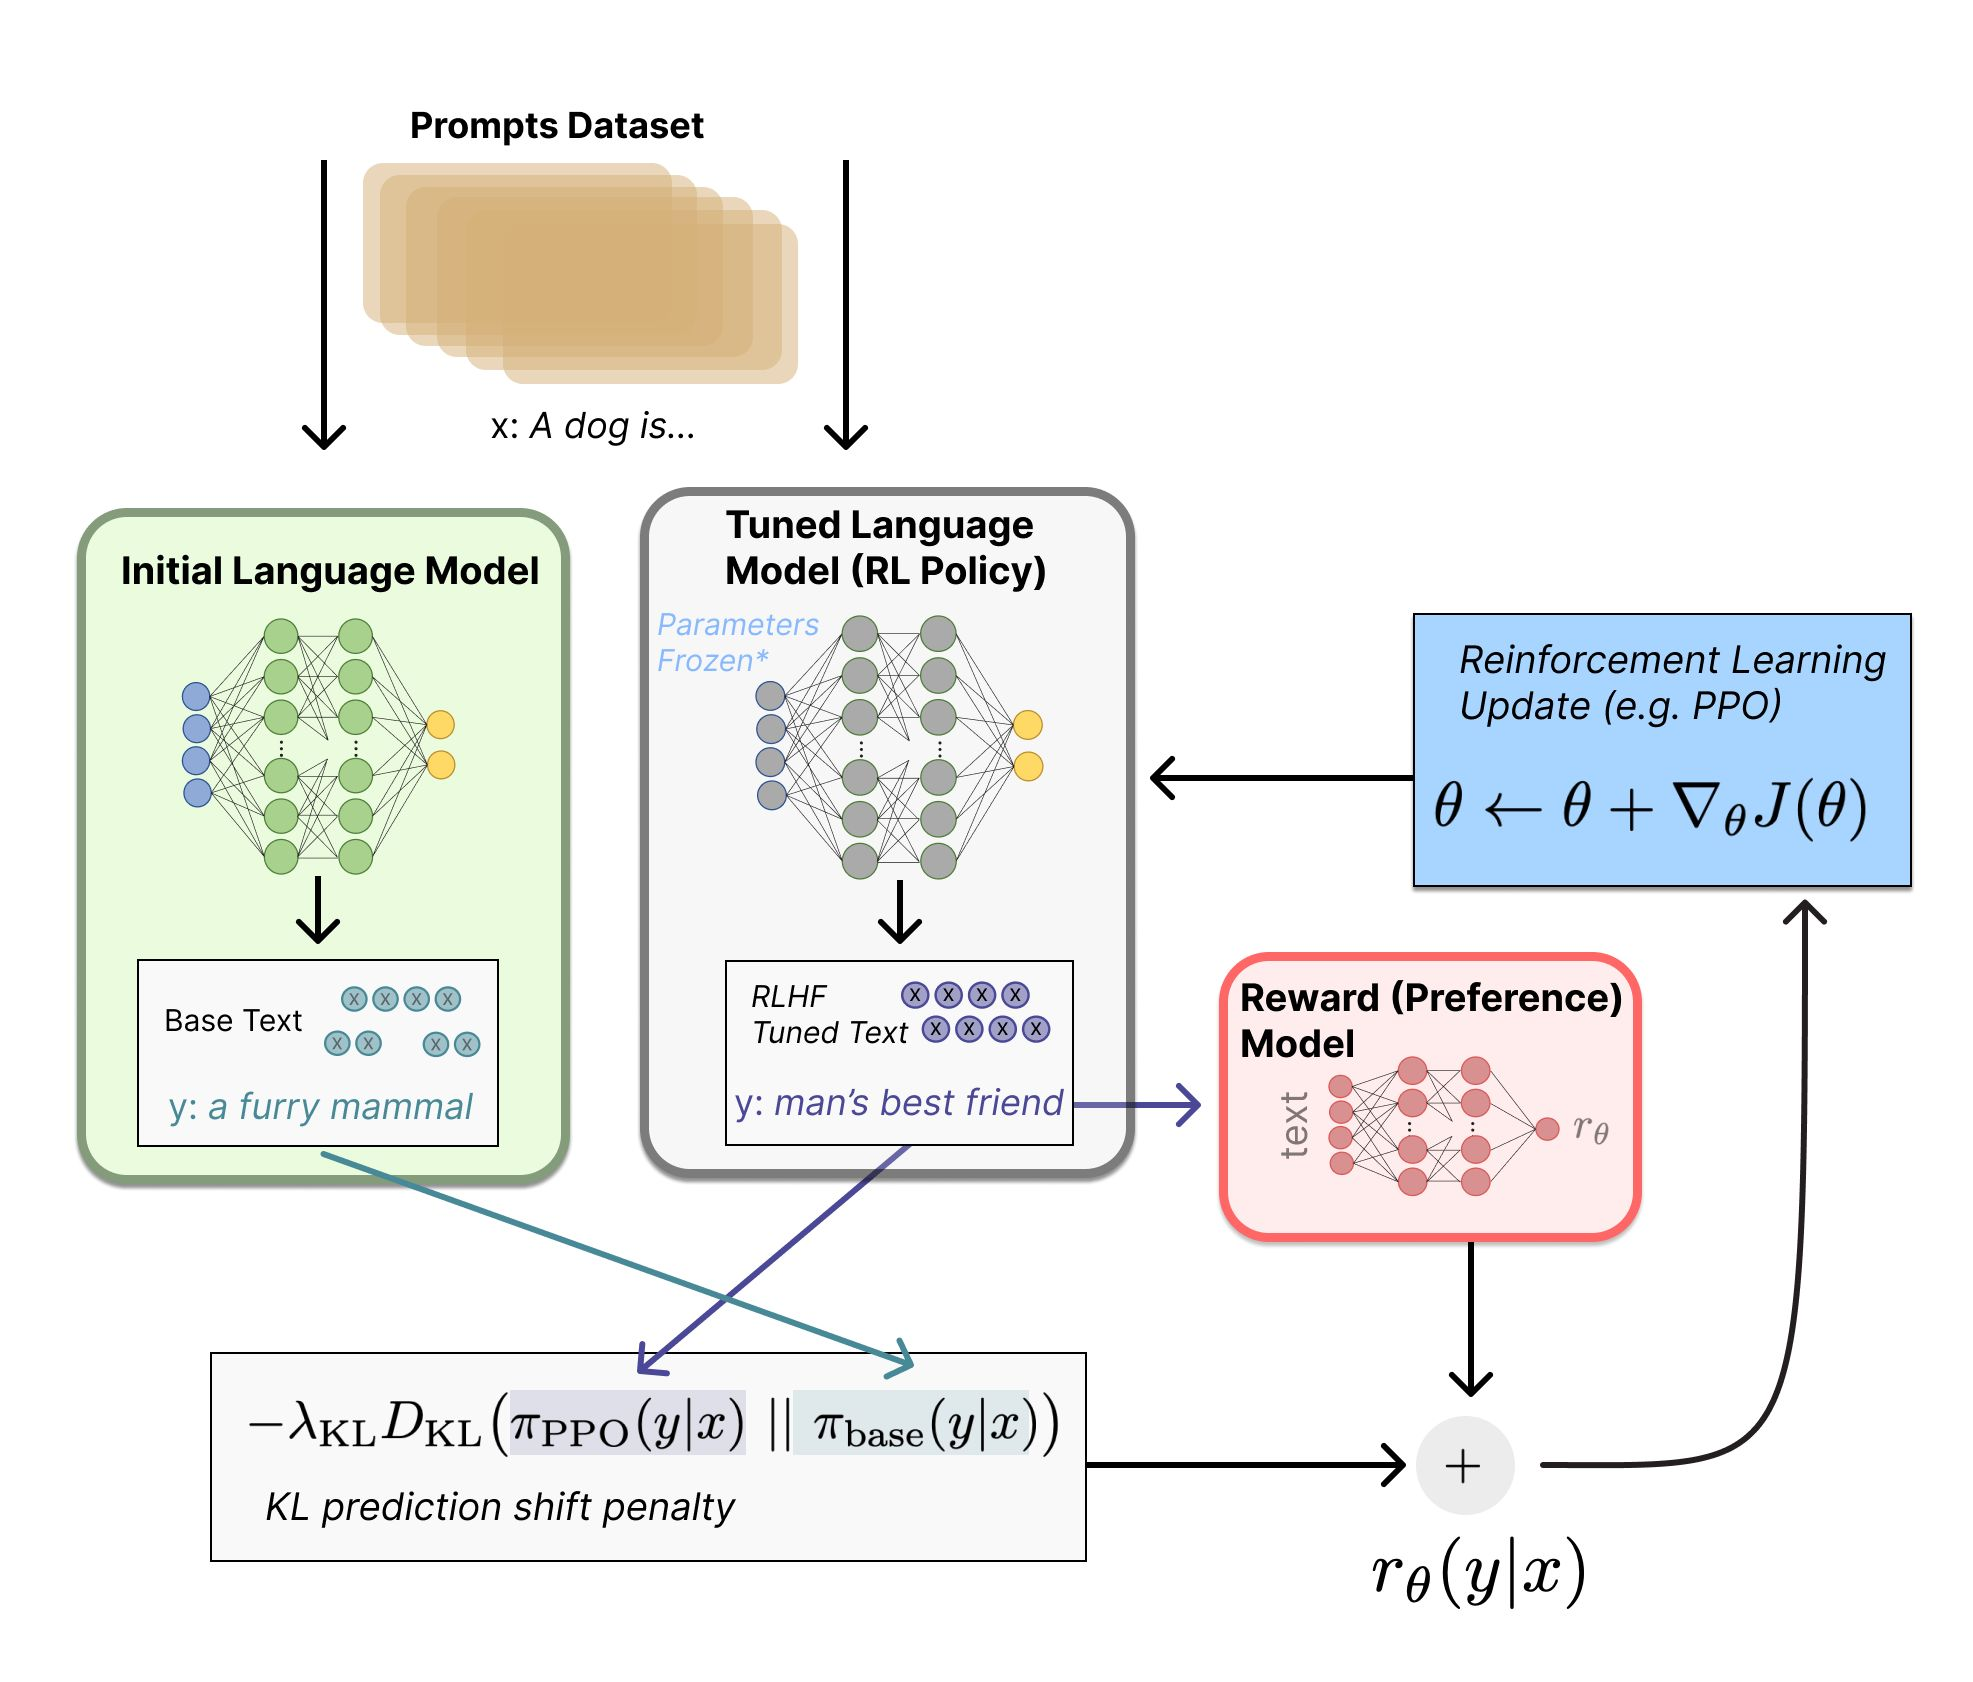
\includegraphics[scale = 0.12]{pics/RLHF.png}
        \end{figure}
        Source: \url{https://huggingface.co/blog/rlhf}


\section{GPT-4 (2023)}
\begin{itemize}
\item Last LM of OpenAI \cite{openai2023gpt4}, this time able to include images in the prompt.
\item Still a Transformer LM.
\item Able to pass exams in several disciplines being able to process the images of the questions.
\item From ChatGPT onwards, companies have stopped making public all the details of the construction of their models.
\end{itemize}

\begin{figure}[h]
	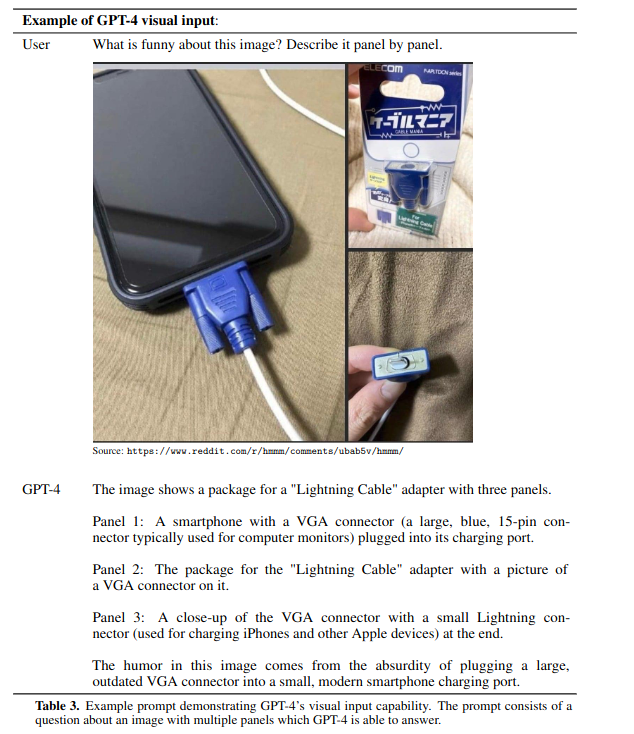
\includegraphics[scale = 0.35]{pics/gpt4.png}
\end{figure}

\section{Instruction Fine-tuning}
\begin{itemize}
\item A more efficient way to fine-tune Large Language Models is Instruction Fine-Tuning  \cite{chung2022scaling}.
\item Idea: collect examples of (instruction, output) pairs across many tasks and finetune an LM.
\item Evaluate on unseen tasks.
\end{itemize}

\begin{figure}[h]
	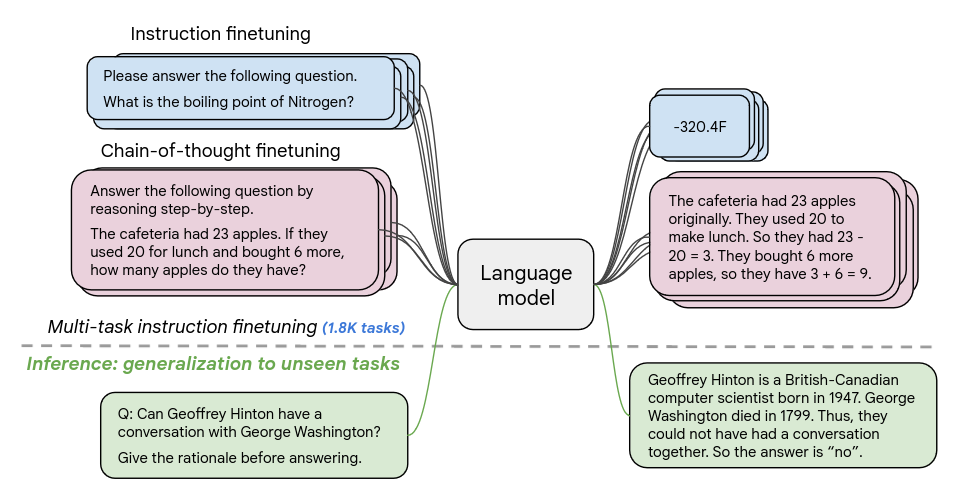
\includegraphics[scale = 0.35]{pics/instructionfinetuning.png}
\end{figure}


\section{Dangers of Large Language Models}
The research community has raised concerns about several dangers associated with Large Language Models \cite{bender2021dangers}.
\begin{itemize}
\item \textbf{Hallucination}: Probabilistic language models can generate fabricated information lacking factual basis.
\item \textbf{Fairness}: These models can perpetuate biases present in the training data, including toxic language, racism, and gender discrimination.
\item \textbf{Copyright infringement}: Large language models may violate copyright laws by reproducing content without proper authorization.
\item \textbf{Lack of transparency}: The complex nature of these models makes it difficult to interpret their predictions and understand the reasoning behind specific responses.
\item \textbf{Monopolization}: The high costs of training these models create barriers for non-big-tech companies to compete.
\item \textbf{High carbon footprint}: The energy-intensive training process of these models contributes to a significant carbon footprint.
\end{itemize}


\section{Large Language Models Time-line}
\begin{itemize}
\item As of today (2023), the development of new Large Language Models continues uninterrupted.
 \begin{figure}[h]
        	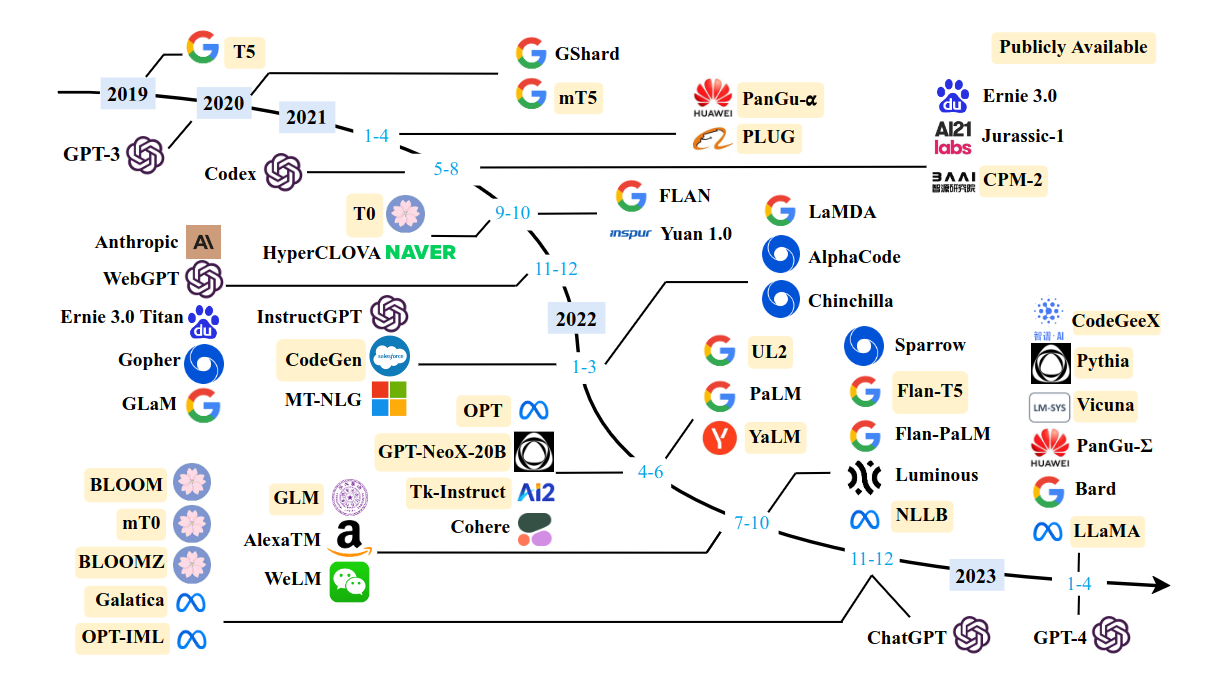
\includegraphics[scale = 0.33]{pics/llmtimeline.png}
        \end{figure}
\item A timeline of existing large language models (having a size larger than 10B) in recent years \cite{zhao2023survey}.
\end{itemize}



\section{Prompt Engineering}
\begin{itemize}
\item Prompt engineering is a new discipline for developing and optimizing prompts to efficiently use language models (LMs).
\end{itemize}
 \begin{figure}[h]
        	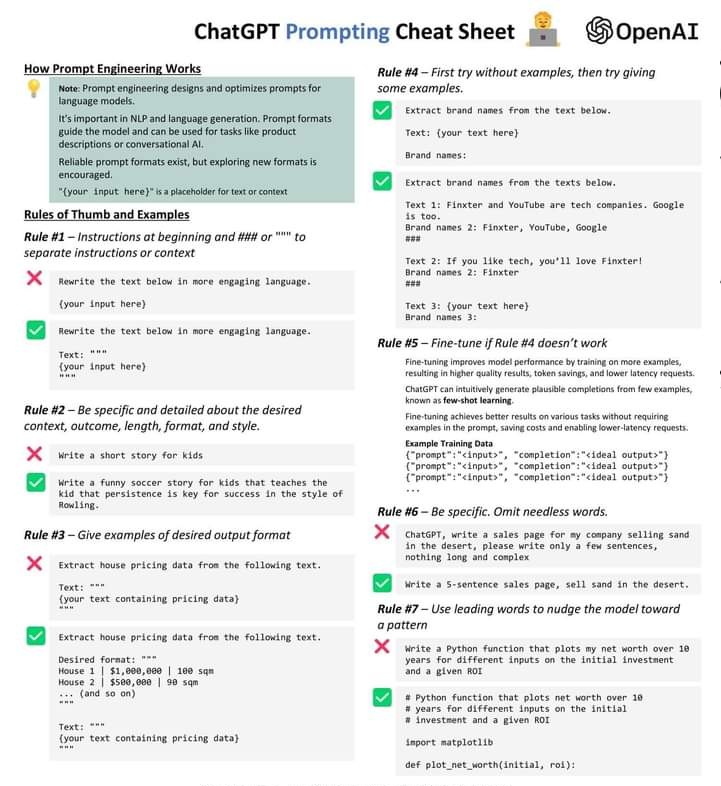
\includegraphics[scale = 0.33]{pics/prompting.png}
        \end{figure}



\section{Conclusions}
\begin{itemize}
\item The growth in the size and power of language models has accelerated dramatically.
\item It is very difficult to predict what they will do in the future.
\item What can we predict with confidence?
\item There will be an overload of generative models for multiple formats (text, code, image, video, virtual realities).
\item There will be a plethora of agents/programs that act and make decisions by interacting with these models (medical appointments, investments, travel).
\end{itemize}

